\section{Motivation}
\label{sec:motive}

\begin{figure}
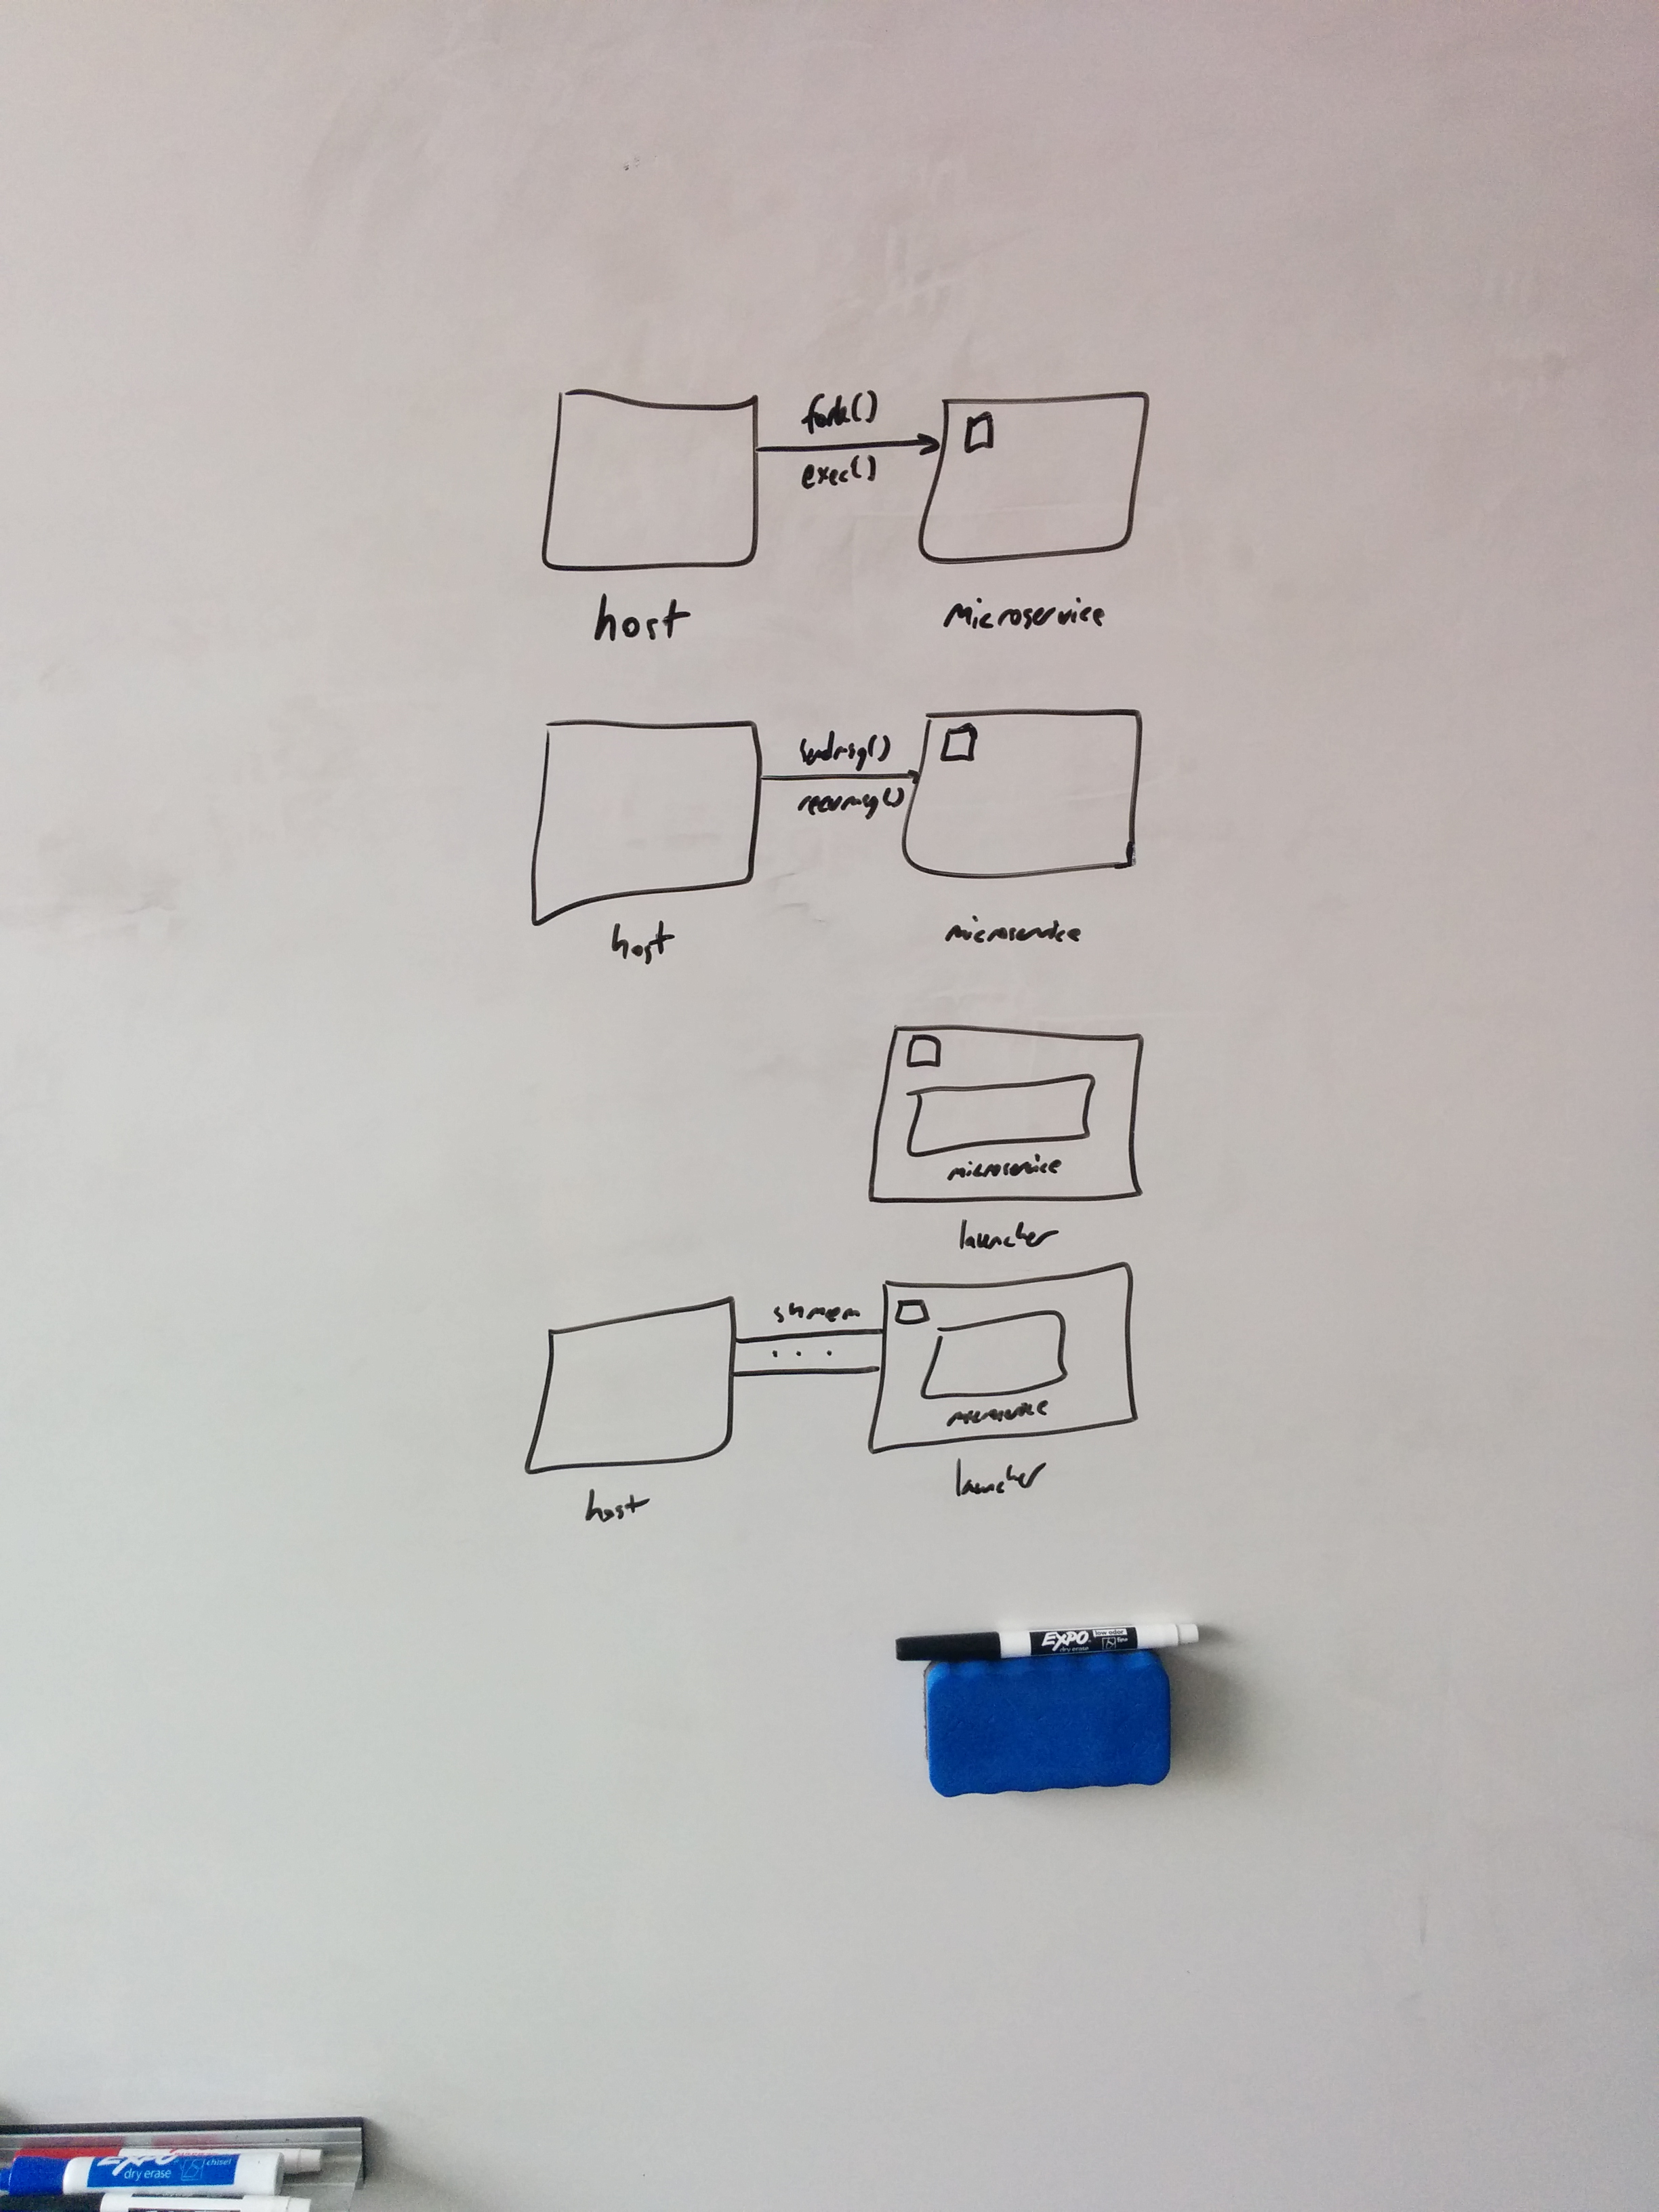
\includegraphics[width=\columnwidth]{figs/IMG_20180125_135549}
\caption{System designs whose invocation latencies we compared}
\label{fig:invocationdesigns}
\end{figure}

We begin our study by comparing the local invocation latencies of a few different possible microservice models.
Traditional serverless platforms spawn a container for each microservice [CITATION NEEDED. OpenLambda?].
To get an approximate lower bound on this latency, we model such systems by executing a process using \texttt{fork}()-\texttt{exec}() each time a request needs to be processed (Figure \ref{fig:invocationdesigns}a).
Having modeled the latency of invoking cold traditional microservices, we consider the cold case, establishing a lower bound by assuming that the processes of all recently executed microservices are kept resident.
Because there are so many processes loaded in this model, they cannot all be running when not in use; as such, we need to use an operating system provided IPC mechanism to wake up the appropriate microservice.
Unix's primary IPC mechanisms exhibit comparable latencies [CITATION NEEDED], so we choose to send UDP datagrams over loopback.
Microservices that aren't currently working spend their time unscheduled, blocked on a \texttt{recv()} system call (Figure \ref{fig:invocationdesigns}b).

We also consider the following design that contrasts with contemporary serverless designs:
Collect groups of microservices into shared \textbf{worker processes} that are constantly running.
If we schedule one such process per physical CPU, they can spend any (rare) time that isn't consumed by user work polling for the next job to arrive (Figure \ref{fig:invocationdesigns}c).
In this way, we expect to be able to achieve significantly lower invocation latencies.
We propose worker processes that use the system's dynamic linker to load user jobs packaged as shared object files.
As before, we can model the behavior of a hot system by keeping the libraries loaded between invocations (Figure \ref{fig:invocationdesigns}d).

Figure \ref{fig:motive} shows the invocation latences of these configurations for various numbers of ``distinct'' microservices (complete copies of the executable or shared library file) on a socket with 14 cores dedicated to the microservices.

\solb{Memory footprint discussion should go here.}

\begin{figure}
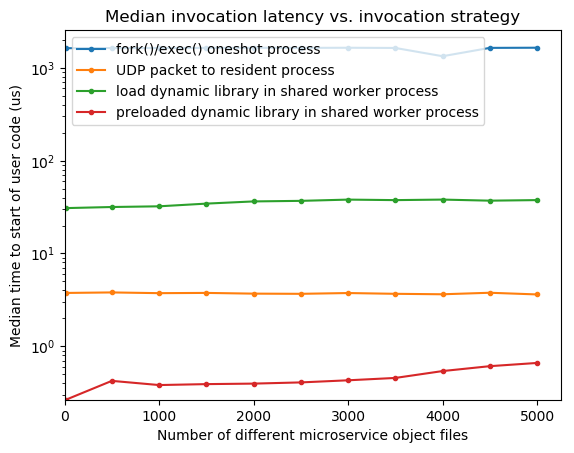
\includegraphics[width=\columnwidth]{figs/2017-01-31-motivation_numfuns-latency_log}
\caption{Median one-way invocation latencies of the four approaches}
\label{fig:motive}
\end{figure}

\solb{I'm planning to run this for various core counts as well, and to look at the memory usage.}
